% Chapter Template
\chapter{Tensor Decomposition} % Main chapter title
\label{Chapter4}
\def \path	{Figures/C4}

In this chapter the main mathematical tools for the manipulation of tensors are introduced. 
Following, we will see how to apply these operators to decompose a convolutional layer through two different techniques, effectively exploring the state-of-the-art methods of low-rank approximation presented in Chapter 2.

%--------------------------------------------------------------------
%	SECTION 1
%--------------------------------------------------------------------
\section{Background}}
\label{sec:bg}
%% intro 
A tensor is a geometric object that generalizes all the structures usually defined in linear algebra to the \emph{n}-dimensional space. As such, they can be defined as \emph{n}-dimensional arrays. 

In fact, recalling that a vectors basis is a set of linearly independent vectors with which we can represent every other vector in the correspondent vector space, a general vector $v$ can be defined as \emph{n}-dimensional array of length \emph{n}. In the same way, we can define \emph{order} (or way) of a tensor the dimensionality of the array needed to represent it with respect to this basis, or the number of indices needed to label a component of that array. 

Thus, an \emph{k-th} order tensor in an \emph{n}-dimensional space is a mathematical object that has \emph{n} indices and $n^k$ components; each index ranges over the number of dimensions of the space.
\newline 

A third-order tensor is showed in \ref{fig:tensor}. 

\begin{figure}[h!]
 \centering
 \includegraphics[width=0.4\textwidth]{\path/tens.png} 
 \caption{A third order tensor.}
 \label{fig:tensor}
\end{figure}

\pagebreak
\subsection{Tensor rank} 
\label{subsec:tensor-rank}
Intuitevely, a scalar would be a tensor of \emph{order 0}; a vector of \emph{order 1}; a matric of \emph{order 2} and so on. 

The intuitive definition can also be used using "\emph{rank}" instead of order, but that may be somewhat misleading since there is a subtle difference. To avoid confusion, the following definitions are introduced: 
\begin{itemize}
  \item a tensor of \emph{rank}-1 (or a decomposable tensor \parencite{tensor-hackbusch2012}) is a tensor that can be written as a product of tensors of the form: 
  \begin{equation}
  \label{eq:rank1-tens}
    T = a \circ b \circ \ldots \circ d  
  \end{equation}   
  
  \item The \emph{rank} of a tensor $X$ is the minimum number of rank-1 tensor that sum to $X$.

\end{itemize}

The product used in \ref{eq:rank1-tens} is an outer product for vectors and will be defined in details in the coming section. 

\subsection{Tensor fibers \& slices}
Tensor fibers are very intuitive to represent visually but not as easy to explain. \\
Let $A(i,j,k)$ be a third-order tensor. The mode-1 fiber of index $s,t$  of $A(i,j,k)$ contains all the elements of A, which have the $j=s$ and $k=t$. 
\\
Intuitively, the \emph{i}-fiber is the "column" that is obtained by fixing one index. Conversely, a tensor \emph{slice} is instead obtained by fixing two indeces. It becomes immediately clear when observing figure \ref{fig:tensor-fibers}. The three different ways in which it is possible to orient a fiber are called \emph{tensor modes}. They are very important to define some basic tensor operation. 

\begin{figure}[h!]
 \centering
 \includegraphics[width=0.9\textwidth]{\path/tensor-mode.jpg} 
 \caption{Fibers and slices of a tensor according to each mode.}
 \label{fig:tensor-fibers}
\end{figure}

\pagebreak
To give another cue on the above, here is a snippet code to index fibers and slices in Python: 
\begin{lstlisting}[language={Python}]
In [13]: tensor = numpy.arange(24).reshape(2,3,4) 
In [14]: tensor
Out[14]: 
array([[[ 0,  1,  2,  3],
        [ 4,  5,  6,  7],
        [ 8,  9, 10, 11]],

       [[12, 13, 14, 15],
        [16, 17, 18, 19],
        [20, 21, 22, 23]]])


In [18]: tensor[:,0,0]
Out[18]: array([ 0, 12])  #Fiber

In [16]: tensor[0,:,:]
Out[16]: 
array([[ 0,  1,  2,  3],
       [ 4,  5,  6,  7],
       [ 8,  9, 10, 11]]) #Slice 

In [17]: 

\end{lstlisting}


Tensors are extensively used in many applications \parencite{WTensor} to modelize multi-dimensional data. In the CNN scenario, a CONV layer with $\mathcal{W}$ weights is defined through a tensor of size: 
\begin{equation}
\label{eq:conv-tensor}
  dim(\mathcal{W})  = [T \times S \times D \times D]
\end{equation}

where, 
\begin{itemize}
 \item $T$ is the number of output filters
 \item $D$ is the size of the kernel of the convolution 
 \item $S$ is the number of input filters 
\end{itemize}

In pure mathematical terms, there exist a lot of different methods to decompose a tensor. In section \ref{sec:tensor-math} the formal tools to wield tensors are given and in section \ref{sec:cpd-application}  the application of these methods to convolutional layers are presented. 

\subsection{Singular value decomposition}
%% SVD Applied on Fully Connected layer 
In order to understand better how a tensor decomposition work and its properties, it is necessary to introduce the \emph{singular value decomposition} (SVD) for matrices. 

Let $M$ be a matrix $\in \mathbf{F}$ of size $m \times n$, the SVD is given by:
\begin{equation}
\label{eq:svd}
   M = U \Sigma V^*
\end{equation}

Where $U$ and $V$ are an $m \times m$ and $n \times n$ unitary matrix respectively. In the case of $\mathbf{F}= \mathbf{R}$, $U$ and $V$ are also orthogonal matrices. $V^∗$ is the conjugate transpose of $V$.  $\Sigma$ is a \emph{diagonal} matrix with non-negative real numbers, which holds the singular values of $M$ in its diagonal. 


A thorough explanation of the above terms is required, so the following definitions must be kept in mind: 
\begin{itemize} 
 \item A \emph{diagonal} matrix is a matrix whose values are all zero except for those on the diagonal. A special case of diagonal matrix is an \emph{identity} matrix, where all these diagonal elements are equal to 1. 
 
 \item Given a matrix $M$, the \emph{transpose} is an operator that flips $M$ over its diagonal producing another matrix $M^T$ as a result, whose column and rows indices are therefore also switched. Hence, the rows of $M$ becomes the columns of $M^T$ and viceversa. 
 
 \item Given a matrix $M \in \mathbf{C}$, its \emph{complex conjugate}, $\bar{M}$, is the conversion of each element $m_{i,j}$ to its conjugate i.e., the real part are the same while the imaginary part have opposite sign and same magnitude. 
 
 \item A \emph{conjugate transpose} is a matrix $M^*$ who's been obtained by first transposing $M$ and then taking the \emph{complex conjugate} of each entry. Also, the following properties holds: 
 		$$
 		M^* = \bar{(M)}^T = \bar{M*T}
 		$$  
 
 \item A quadratic matrix $M$ is said to be \emph{unitary} if $MM^* = M*M = I$, where $I$ is the identity matrix. In the case $M \in \mathbb{R}$ the matrix is called \emph{orthogonal} and it satisfies the equivalence $MM^T = M^TM = I$. 
 
 \item An \emph{orthogonal} matrix has rows and columns that are unitary or orthogonal between each other, respectively. 
 
 \item A non-negative real number $\sigma$ is a singular value for $M$ of a space $F^{m \times n}$ if and only if there exist unit-length vectors  $u \in \mathbf{F}^m, \, v \in \mathbf{F}^n$ such that $Mv=\sigma u$ and $M^*u=\sigma v$. The vectors $u$ and $v$ are called left-singular and right-singular vectors for $\sigma$ respectively. 

\end{itemize}

Recalling the SVD definition \ref{eq:svd}, the $\m \times n$ rectangular matrix $\Sigma$ holds the  \emph{singular values} (the square roots of the non-zero \emph{eigen-values})  $\sigma_i \: i=1, \ldots, k$ of $M$ on its diagonal. The first $k = min(m,n)$ columns of $U$ and $V$ are, respectively, left-singular vectors and right-singular vectors for the corresponding singular values. Consequently, the SVD theorem implies that: 
\begin{itemize}
	\item An $m \times n$ matrix $M$ has at most $k$ distinct singular values; 
    \item It is always possible to find a unitary basis $U$ for $\mathbf{F}^m$ with a subset of basis vectors spanning the left-singular vectors of each singular value of $M$; 
    
    \item It is always possible to find a unitary basis $V$ for $\mathbf{F}^n$ with a subset of basis vectors spanning the right-singular vectors of each singular value of $M$.
\end{itemize} 


\subsection{SVD Applications}
The SVD factorization is useful in  many fields of research. It can be used to solve the \emph{linear least-squares} and the \emph{total least-squares} problems; it is widely used in statistics where it is related to \emph{principal component analysis} (PCA); it's successfully used in signal processing and pattern recognition. SVD is also fundamental in \emph{recommender systems} to predict people's item ratings \parencite{recsys1} \parencite{recsys2}; for instance, Netflix has launched a global competition to find the best implementation of SVD for clusters to improve its collaborative filtering technique \parencite{recsys3-netflix}. The main area of interest of SVD for convolutional neural networks is that of \emph{low-rank matrix approximation} and image processing. 

In fact, SVD can be thought of as decomposing a matrix into a \emph{weighted, ordered} sum of separable matrices. Separable here means exactly the same concept introduced for tensors in section \ref{subsec:tensor-rank} i.e., a matrix $A$ can be written as an outer product of two vectors $A = u \circ v$. More precisely, the matrix can be factorized as: 
\begin{equation}
  M = \sum_i A_i = \sum_i \sigma_i U_i \circ V_{i}^{T}  
\end{equation} 

this turns out to be enable a fast convolution computation: 

\begin{equation}
	F = \sum_{i}^{R} \sigma_i(I * U_i)*V_i  
\end{equation}

where I is the input image, $F$ is the resultant feature map and $U_i$ and $V_i$ are i-th column of $U$ and $V$ respectively. 

Note that $\sigma_i$ are the R largest singular values (the other singular values are replaced by zero). Since the number of non-zero $\sigma_i$ correspond exactly to the rank of a matrix, the approximated matrix is thus of rank R. \\
For this purpose, given a matrix $M$, the best method to find a truncated matrix $\tilde{M}$ of rank $R$ that approximates $M$, is to find the solution that minimizes the \emph{frobenius norm} of their difference:
\begin{equation}
\left \| M - \hat{M} \right \|, \quad with \ \hat{M} = \sum_i U_i \circ V_i
\end{equation}

The Eckart-Young theorem \parencite{Weckart} states that the best solution to the problem is given by its SVD decomposition. 

\subsubsection{SVD on CNN}
Given its application to speed up convolution filters, it is not surprising that SVD has been one of the methods used in recent developments on deep CNN compression, as portrayed in chapter \ref{Chapter2}.
In particular, the work of Cheng et al. \parencite{zhang2015SVD} applies an original decomposition scheme which is based on top of SVD. 

Given a conv layer with weights $\mathcal{W} = [T \times S \times d \times d]$, it consists in constructing a bigger matrix $\mathcal{B}$ built with the stack of feature maps, namely spreading the input channels kernels on rows and kernel composing the filter bank on column. Then, it computes the SVD of the so obtained matrix and ... 
 

\subsubsection{SVD on fully-connected layers}
\label{subsec:svd-fc}
Beside convolution, there is another way to leverage on SVD in convnets and that is the fully-connected layers. In practice, fully-connected layers are just plain matrix multiplication plus a bias:
\begin{equation}
\label{eq:fc}
Y = W*X+B 
\end{equation}
where X are the input maps and $W$ is an $m \times n$ matrix that holds the weights of the layer.  

From this observation, a recipe to speed up fully-connected layers can be spotted: 
\begin{enumerate}
	\item compute the truncated SVD of the weight matrix $W$ keeping only the first $\mathit{r}$ singular values; 
	\item substitute the layer with 2 smaller fully-connected ones; 
	\item the first one will have a shape of $[m \times r]$ and no bias; 
	\item the second will have a shape of $[ r \tiems n]$ and a bias equal to its original bias $B$.   
\end{enumerate}

The SVD decomposition of the layer is formalized as follow: 
\begin{equation}
(U_{m \times r} \Sigma_{r \times r} V^T_{n \times t}) X+ B = U_{m \times r} ( \Sigma_{r \times r}V^T_{n \times r} X) + B 
\end{equation}


This way, the total number of weights dropped from $n \times m$ to $r(n+m)$, which is dependent on the choice of the rank of the approximation $r$ and can be significant when $r$ is a much smaller than $min(n, m)$.\\
The first reference of this approach could be find in the \emph{Fast R-CNN} paper \parencit{fast-rcnn}, an efficient implementation of RCNN \parencite{rcnn}, a very famous CNN built for region proposal and object detection. The implementation for Caffe is also available on the author github page, at \parencite{Wgithub-rcnn}.
%--------------------------------------------------------------------
%	SECTION 2
%--------------------------------------------------------------------
\section{Tensor mathematical tools}
\label{sec:tensor-math}

\subsection{Basic operations}
In multi-linear algebra it actually does not exist a method that satisfy all SVD properties for \emph{m-way arrays}, i.e. tensors. However, by taking a closer look at SVD we can formulate two main requirements that a tensor decomposition algorithm should satisfy to be a feasible alternative to SVD in a tensor-world: 
{\begin{enumerate}
	\item a Rank-\textit{R} decomposition
	\item the orthonormal row/column matrices.
\end{enumerate}}

SVD computes both of them simultaneously. Regarding tensors, these properties can be captured separately by two different family of decompositions.

The first property is extended to the multi-linear world by a class of decompositions that fall under the name of \textit{CP decomposition} (named after the two most popular variants, CANDECOMP and PARAFAC). The latter is provided by the Tucker methods (and many other names). For each axes of a tensor, these methods compute the associated orthonormal space. Therefore, Tucker methods are also used in multilinear principal component analysis (PCA). 
\newline 
	
Historically, much of the interest in higher-order SVDs was driven by the need to analize empirical data, expecially in psychometrics, chemometrics and neuroscience \parencite{tensor2009kolda}. As such, these techniques have been rediscovered many times with different names leading to a confused literature. Thus, these methods are often presented in a more practical goal-driven way, rather than through rigourous abstract general theorems, which are in fact rare.\\

Before diving into tensor decomposition algorithms, we need to introduce some fundamental tensor operations: 

\begin{itemize}
	\item \textbf{Tensor unfolding}: Tensor unfolding, also called \emph{matrization}, is an operation that maps a tensor $X$ into a matrix $M$. It is done by taking each mode-\emph{i} fiber of a tensor and lay them down as columns in the resulting matrix. The other modes are handled cyclically. The specified mode will be the first mode of the matrix i.e., given $X$ of size $I \times J \times K$, the first-mode unfolding will produce a matrix $M$ of size $I \times JK$.

	A simpler way to look at it is by taking the mode-\emph{i} slices and put them one after the other. An example for the a third-order tensor is illustrated in \ref{fig:unfolding}.
	
				
			\begin{figure}[h!]
			 \centering
			 \includegraphics[width=1.0\textwidth]{\path/tensor-unfold.jpg} 
			 \caption{Tensor unfolding or matricization along different modes.}}
			 \label{fig:unfolding}
			\end{figure}
			            

    \item  \textbf{Tensor times matrix: \textit{k}-mode product:} 
            The $k$-mode product of a tensor X $\in \mathbb{R}^{I_{1} \times I_{2} \times \ldots \times I_{N}}$ with a matrix $M \in \mathbb{R}^{J \times I_{k}}$ is written as: 
           \begin{equation}
                \textbf{Y} = \textbf{X} \times_{k} M
           \end{equation}
            The resulting tensor $Y$ is of size $I_{1} \times \ldots \times I_{k-1} \times J \times I_{k+1} \times \ldots \times I_{N}$, and contains the elements:

            $$ 
             y_{i_{1}  \cdots  i_{k-1}  j  i_{k+1}  \cdots  i_{N}} =   \sum_{i_{k} = 1}^{I_{k}} x_{i_{1}  i_{2}  \cdots  i_{N}} a_{ji_{k}}.
            $$
             
             It can be hard to visualize this operation at first, but effectively it boils down to 
             multiply each mode-\textit{k} fiber of X by the matrix M. Looking at \ref{fig:unfolding}, we can also represent the same operation with 
             $ \textbf{Y}_{(i)} = \textbf{X}_{(i)} \cdot M$, being $\mathbf{X}_{(i)}$ the mode-i unfolding of the tensor X.
             


             To simplify things, let \textbf{X} be a 3-mode tensor $\in F^{I \times J \times K}$ and $M$ a matrix $\in F^{N \times J}$, the k-mode product on axis 1 of X and M is:
            
            \begin{equation}
                        \textbf{Y} = \textbf{X} \times_{1} M, Y \in F^{I \times J \times K} 
            \end{equation}
            So each element (\textit{n, j, k}) of Y is obtained by: 
            \begin{equation}
                y_{n,j,k} = \sum_{i} x_{i,j,k}  \cdot  b_{n,j}  
            \end{equation}
            
            A visual example is depicted in \ref{fig:k-mode}.
            
            
			\begin{figure}[h!]
			 \centering
			 \includegraphics[width=1.0\textwidth]{\path/k-mode.png} 
			 \caption{An example of a \emph{k}-mode product i.e., a tensor-matrix multiplication of a 3-dimensional tensor.}}
			 \label{fig:k-mode}
			\end{figure}
                        
            Few interesting properties of the k-mode product are: \\
            \begin{itemize}
                \item  $\tensor{X} \times_{m} A \times_{n} B = \tensor{S} \times_{n} B \times_{m} A$ if $n \neq m$ \\
                
                \item  $X \times_{n} A \times_{n} B = \tensor{X} \times_{n} (BA)$ $\neq \tensor{X} \times_{n} B \times_{n} A$.
            \end{itemize}

    
    \item \textbf{Tensor times vector}: 
       Given the same matrix X, the tensor-vector multiplication on the \textit{i}-axis is defined as:
       \begin{equation}
           \textbf{Y} = \textbf{X} \times_1 v, \textbf{Y} \in \mathbb{}
       \end{equation}

        with each element $y_{j,k}$: 
        \begin{equation}
            y_{j,k} = \sum x_{i,j,k} \cdot a_i
       \end{equation}
       
       An example is illustrated in \ref{fig:tensor-to-vec}.
		 
		 \begin{figure}[h!]
		 \centering
		 \includegraphics[width=1.0\textwidth]{\path/tensor-vec.png} 
		 \caption{An example of a tensor-vector product.}}
		 \label{fig:tensor-to-vec}
		\end{figure}





        
    \item \textbf{Matrix Kronecker product}: 
       A Kronecker product of two matrices $A \in \mathbf{R}^{M \times N}$ and $B \in \mathbf{R}^{P \times Q}$
       is defined as: 
        \begin{equation} 
        A\otimes B = \begin{bmatrix} a_{11} B & \cdots & a_{1n}B \\ \vdots & \ddots & \vdots \\ a_{m1} B & \cdots & a_{mn} B \end{bmatrix}
        \end{equation}
        
        and more explicitly: 
\begin{align*}
\centering
   \mathbf{A}\otimes\mathbf{B} = \begin{bmatrix}
   a_{11} b_{11} & a_{11} b_{12} & \cdots & a_{11} b_{1q} &
                   \cdots & \cdots & a_{1n} b_{11} & a_{1n} b_{12} & \cdots & a_{1n} b_{1q} \\
   a_{11} b_{21} & a_{11} b_{22} & \cdots & a_{11} b_{2q} &
                   \cdots & \cdots & a_{1n} b_{21} & a_{1n} b_{22} & \cdots & a_{1n} b_{2q} \\
   \vdots & \vdots & \ddots & \vdots & & & \vdots & \vdots & \ddots & \vdots \\
   a_{11} b_{p1} & a_{11} b_{p2} & \cdots & a_{11} b_{pq} &
                   \cdots & \cdots & a_{1n} b_{p1} & a_{1n} b_{p2} & \cdots & a_{1n} b_{pq} \\
   \vdots & \vdots & & \vdots & \ddots & & \vdots & \vdots & & \vdots \\
   \vdots & \vdots & & \vdots & & \ddots & \vdots & \vdots & & \vdots \\
   a_{m1} b_{11} & a_{m1} b_{12} & \cdots & a_{m1} b_{1q} &
                   \cdots & \cdots & a_{mn} b_{11} & a_{mn} b_{12} & \cdots & a_{mn} b_{1q} \\
   a_{m1} b_{21} & a_{m1} b_{22} & \cdots & a_{m1} b_{2q} &
                   \cdots & \cdots & a_{mn} b_{21} & a_{mn} b_{22} & \cdots & a_{mn} b_{2q} \\
   \vdots & \vdots & \ddots & \vdots & & & \vdots & \vdots & \ddots & \vdots \\
   a_{m1} b_{p1} & a_{m1} b_{p2} & \cdots & a_{m1} b_{pq} &
                   \cdots & \cdots & a_{mn} b_{p1} & a_{mn} b_{p2} & \cdots & a_{mn} b_{pq}
\end{bmatrix} 
\end{align*}
        
    
    \item \textbf{Outer product}: If we take the \emph{Kronecker product for matrices} definition and apply it to vectors, we obtain the outer product: \\
        
        \begin{align}
            \mathbf{a} \circ \mathbf{b} = \mathbf{a} \mathbf{b}^\mathrm{T}
            = \begin{bmatrix}a_1 \\ a_2 \\ a_3 \\ a_4\end{bmatrix}
            \begin{bmatrix}b_1 & b_2 & b_3\end{bmatrix}
            = \begin{bmatrix}a_1b_1 & a_1b_2 & a_1b_3 \\ a_2b_1 & a_2b_2 & a_2b_3 \\ a_3b_1 & a_3b_2 & a_3b_3 \\ a_4b_1 & a_4b_2 & a_4b_3\end{bmatrix}.
        \end{align}

        Let $a \in \mathbf{R}^I$, $b \in \mathbf{R}^J$  $c \in \mathbf{R}^K$ be three vectors. Computing the outer 
        product ($a  \circ  b$) of two of them will result in a matrix, as showed above. Proceeding in this way is easy to show that an outer product of 3-vectors will result in a 3-dimensional tensor, as illustrated in \ref{fig:tensor-outer-product}.
        
        This comes in handy the other way around: a rank-1 tensor can be decomposed into 3 vectors. As we will see in the following sections, this operation is fundamental for tensor decomposition.\\
        Another interesting way to look at it is that the outer product operation “◦” is a way of combining a tensor of $d1$-order and a tensor of $d2$-order to obtain a tensor of order-$(d1+d2)$.
        
         \begin{figure}[h!]
 		\centering
 		\includegraphics[width=0.7\textwidth]{\path/tensor-vec3.jpg} 
 		\caption{Representation of third-order tensor with an outer product of vectors.}
 		\label{fig:tensor-outer-product}
		\end{figure}

    \item \textbf{Matrix Khatri-Rao product}: given two matrices $A \in \mathbf{R}^{M \times N}$ and $B \in            \mathbf{R}^{P \times R}$ is defined as: 
        \begin{equation}
            A \odot B = [a_1 \otimes b_1, a_2 \otimes b_2, \ldots, a_N \otimes b_R] \in \mathbf{R}^{MN \times R}
        \end{equation}
        
        Note that the Kronecker matrix operation returns the same number of elements of the Khatri-Rao product, but while the former produce a matrix, the latter is shaped into a vector.   
\end{itemize}

\newpage
\subsection{Tucker Decomposition}
The Tucker decomposition is a way to write a tensor of size $I_1 \times I_2 \times \ldots \times I_N$ as the multi-linear tensor-matrix product of a \emph{core} tensor $\mathbf{G}$ of size $R_1 \times R_2 \times \cdots \times R_N$ with $N$ factors $A^{(n)}$ of size $I_n \times R_n$:

\begin{equation}
\label{eq:tucker-general}
    \mathrm{X} = \mathbf{G} \times_{1} A^{(1)} \times_{2} A^{(2)} \times_{3} \ldots \times_{N} A^{(N)}
\end{equation}
where $\times_k$ is the k-mode product introduced before. 
\newline 
 
To make this definition a little bit more intuitive, let X be a third-order tensor $\in \mathbf{R}*{I \times J \times K)$, then the Tucker decomposition is defined as :

\begin{equation}
\label{eq:tucker-3}
	X = \mathbf{G} \times_1 A \times_2 B \times_3 C  = \sum_r \sum_s \sum_t \mathit{\sigma}_{r,s,t} u_r \circ v_s \circ w_t 
\end{equation}
 
 where $A$ is a $I \times R$ matrix, $B$ is a $J \times S$ matrix, $C$ is a $K \times T$ matrix and $\mathbf{G}$ is a $R \times S \times T$-tensor with $R < I$, $S < J$ and $T < K$. 
\newline


An example of third-order tensor Tucker decomposition is depicted in figure \ref{fig:tucker-dec}. 


\begin{figure}[h!]
 \centering
 \includegraphics[width=1.0\textwidth]{\path/tucker-dec.jpg} 
 \caption{A Tucker decomposition of a three-modes tensor}
 \label{fig:tucker-dec}
\end{figure}



A matrix representation of the Tucker tensor is given by the following equations: 
\begin{equation}
  X_{(1)} = A\mathbf{G}_{(1)} (C \otimes B)^T
\end{equation}

\begin{equation}
  X_{(2)} = B\mathbf{G}_{(2)} (C \otimes A)^T
\end{equation}

\begin{equation}
  X_{(3)} = A\mathbf{G}_{(3)} (B \otimes A)^T
\end{equation}

and it is also possible to unfold it into a vector: 
\begin{equation}
 vec(X) = (C \otimes B \otimes A) vec(\mathbf{G})
\end{equation}

It is worth noting that we can see a Tucker decomposition as an SVD in each dimension, being $\mathcal{G}$ the singular value tensor and $A, B, C$ the matrices with the singular vectors of each dimension.

 We have already seen how SVD can be useful in reducing complexity in fully-connected layers \ref{subsec:svd-fc}; therefore it's legitimate to presume that the Tucker decomposition can have a meaningful impact on the filter maps in convolutional layers. \\
 Moreover, from chapter 3 we can recall that convolutional filters expose a \emph{parameter sharing} design. Hence it is intuibile that those filters will have some related parameters and thus feasible to a good factorization.  

\subsubsection{HO-SVD}
\label{subsec:hosvd}
As the \emph{Higher-order singular value decomposition} was studied in many scientific fields, it is historically referred in different ways:  multilinear singular value decomposition, m-mode SVD, or cube SVD, and it is often incorrectly identified with a Tucker decomposition. 

HOSVD is actually a specific orthogonal version of the Tucker decomposition. To put it in other words, it is a specialized algorithm to compute the Tucker decomposition. HOSVD involves solving each \emph{k}-mode matricized form of the specific tensor \parencite{WTucker}, relying on the following equivalence: \\

\begin{eqnarray}
	\centering
	Y &=& X \times_{1} A^{(1)} \times_{2} A^{(2)} \times_{3} \ldots \times_{N} A^{(N)} \nonumber\\
	\Leftrightarrow \quad Y_{(k)} &=& A^{(k)} X_{(k)} \left(A^{(N)} \otimes \cdots \otimes A^{(k+1)}   \otimes A^{(k-1)} \otimes \cdots A^{(1)} \right)^T. \nonumber
	\end{eqnarray}

The algorithm steps follow: 
\begin{eqnarray}
&\,&\mathrm{for}\, k = 1, 2, ..., N \,\mathrm{do} \nonumber\\
&\,&\quad A^{(k)} \leftarrow \,\mathrm{left\,orthogonal\,matrix\,of\,SVD\,of}\,X_{(k)} \nonumber\\
&\,&\mathrm{end\,for} \nonumber\\
&\,&G \leftarrow X \times_{1} (A^{(1)})^T \times_{2} (A^{(2)})^T \times_{3} \cdots \times_{N} (A^{(N)})^T  \nonumber
\end{eqnarray} 

This approach may be regarded as one generalization of the matrix SVD, because:
\begin{itemize}
	\item each matrix $\mathit{A}^k$ is an ortoghonal matrix 
	\item Two subtensors of the core tensor $\mathbf{G}$ are orthogonal, i.e. $\left \langle \mathbf{G}_p , \mathbf{G}_q \right \rangle \quad if \quad p \neq q$
	\item the subtensors in the core tensor $\mathbf{G}}$ are ordered according to their Frobenius norm, i.e. $\left \| \mathbf{G}_1 \right \|  \geq  \left \| \mathbf{G}_2 \right \| \geq \ldots  \geq \left \| \mathbf{G}_n \right \|_{\: for \: n=1,\ldots,N} $
\end{itemize}
	
A nice visualization of HOSVD is given in figure \ref{fig:hosvd}. The tensor $\mathbf{G}$ is said to be \emph{"ordered"} and \emph{"all-ortoghonal"}. For further explanation see \parencite{multilinear}. 

\begin{figure}[h!]
 \centering
 \includegraphics[width=1.0\textwidth]{\path/HOSVD.jpg} 
 \caption{An Higher Order SVD of a third-order rank-(R1-R2-R3) tensor and the different spaces, from Tensorlab \parencite{WTensorlab}.}
 \label{fig:hosvd}
\end{figure}

\subsubsection{Higher order orthogonal iteration}
As for SVD, it is important to notice that HOSVD can be used to compress $X$ by truncating the matrices $A(k)$. The problem with respect to matrices though, is that a truncated HOSVD is known not to give the best fit. However, as a logical consequence of two concepts that have been introduced earlier, an iterative algorithm to find the best solution can be proposed.
\newline
In fact, putting together the Eckart-Young theorem for the \emph{Frobenius} norm and the HOSVD depicted above will result in an iterative optimization known as Higher-Order Orthogonal Iteration or \emph{HOOI}. 
\newline

HOOI finds the optimal approximation $\hat{X}$ with respect to the Frobenius norom loss by, essentially, iterating the alternating truncation and SVD. Thus, enforcing $A(k)$ to have $r_k$ columns, the HOOI solution is defined by the following algorithm: 
\begin{eqnarray}
&\,&\mathrm{initialize\,via\,HOSVD} \nonumber\\
&\,&\mathrm{while\,not\,converged\,do} \nonumber\\
&\,&\quad \mathrm{for}\, k = 1, 2, ..., N \nonumber\\
&\,&\quad\quad Y \leftarrow X \times\subscript{1} (A^{(1)})^T \times\subscript{2} \cdots \times\subscript{k-1} (A^{(k-1)})^T \times\subscript{k+1} (A^{(k+1)})^T \times\subscript{k+2} \cdots \times\subscript{N} (A^{(N)})^T  \nonumber\\
&\,&\quad\quad A^{(k)} \leftarrow r\subscript{k}\,\mathrm{leading\,left\,singular\,vectors\,of}\,Y\subscript{(k)} \nonumber\\
&\,&\quad \mathrm{end\,for} \nonumber\\
&\,&\mathrm{end\,while} \nonumber\\
&\,&G \leftarrow X \times\subscript{1} (A^{(1)})^T \times\subscript{2} (A^{(2)})^T \times\subscript{3} \cdots \times\subscript{N} (A^{(N)})^T  \nonumber\\
\end{eqnarray}


\subsection{Canonical Polyadic Decomposition}
\begin{comment}
$\tensor{A} \otimes \tensor{B}$ denote the outer product between an $N\th$-order tensor $\tensor{A}$ and an $M\th$-order tensor $\tensor{B}$, then $\tensor{A} \otimes \tensor{B}$ is the $(N+M)\th$-order tensor defined by $(\tensor{A} \otimes \tensor{B})_{i_1\cdots i_N\,j_1\cdots j_M} = a_{i_1\cdots i_N} \cdot b_{j_1\cdots j_M}$. 
\end{comment}
%% rivedere %% 
The Polyadic Decomposition (PD) \parencite{tensor2009kolda} approximates a tensor with a sum of $R$ rank-one tensors. If the number of rank-one terms $R$ is minimal, then $R$ is called the rank of the tensor and the decomposition is called minimal or \emph{canonical} (CPD). \\
For any other arbitrary \mathit{rank-r}, the decomposition is often referred to as CANDECOMP/PARAFAC (CP). As we will discover later, selecting the perfect rank is an \emph{NP-Hard} problem. Hence, from now on we will refer to this decomposition as CP. \newline 

Recall the outer product between vectors introduced in section \ref{sec:tensor-math}.
Let $\vec{a}$, $\vec{b}$ and $\vec{c}$ be nonzero vectors in $\mathbf{R}^{n}$, then $\vec{a} \circ \vec{b} \equiv \vec{a}\cdot \vec{b}^{\T}$ is a rank-one matrix and
$\vec{a} \circ \vec{b} \circ \vec{c}$ is defined to be a rank-one tensor. Let $\ten{T}$ be a tensor of dimensions $I_1 \times I_2 \times \cdots
\times I_N$, and let $\mat{U}^{(n)}$ be matrices of size $I_n \times R$ and $\vec{u}_r^{(n)}$ the $r$\th column of $\mat{U}^{(n)}$,
then:

\begin{equation}
    \ten{T} \approx \sum_{r=1}^{R} \vec{u}^{(1)}_r \circ \vec{u}^{(1)}_r \circ
   \cdots \circ \vec{u}^{(N)}_r.
\end{equation} 

A visual representation of this decomposition in the third-order case is shown
in \ref{fig:cpd}

It's interesting to notice that CPD can be regarded as a special case of a Tucker Decomposition in which the core tensor $\mathbf{G}$ is constrained to be a super-identity I, which is an extension of the identity matrix and has all one's on its superdiagonal and all zero's off the superdiagonal. 




%--------------------------------------------------------------------
%	SECTION 3
%--------------------------------------------------------------------
\section{Application of tensor decompositon on CNN}
\label{sec:cpd-application}
\subsection{Convolutional layer as 4-mode tensors}
Convolutional layers units are organized as 3D tensors (\emph{map stacks}) with two spatial dimensions and the third dimension corresponding to the different maps, or "channels". The most computational demanding operation within CNNs is the generalized - or standard - convolution that maps an input tensor $U(.,.,.)$ of size $X \times Y \times S$ to an output tensor $V(.,.,.)$ of size $(X -d+1 \times (Y-d+1) \times T$ using the following linear mapping: 
\begin{equation}
\label{eq:convolution}
V(x, y, t)= \sum_{i=x-\delta}^{x+\delta} \sum_{j=y-\delta}^{y+\delta} \sum_{s=1}^S K(i-x+\delta, j-y +\delta,s,t) U(i,j,s) 
\end{equation}

Thus it is possible to summarize a convolutional layer with the 4D kernel tensor $K(.,.,.,.)$ of size $d \times d \times S \times T$ where $d$ is the spatial dimension of the 2D convolutional kernel, $S$ and $T$ are the input channels and the output channels dimension respectively. The "half-width" $\frac{d-1}{2}$ is denoted with $\delta$, assuming square shaped kernels and even value of $d$ as it is most often the case. 

\subsection{CP}
Once we have modelized the convolutional kernel, we can actually grasp how the tensor decomposition can be practically applied on a CNN. A rank-$R$ CP-decomposition of a 4D tensor will result in 4 factor matrices $K^n$ with size equals to $I_n \times R$. Therefore, applying this decomposition on $K(.,.,.,.)$ will result in: 

\begin{equation}
\label{eq:cpd-classic}
 \sum_{r=1}^R K^x(i-x+ \delta,r)K^y(j-y+ \delta,r)K^s(s,r)K^t(t,r) 
\end{equation}
where $K^x, K^y, K^s, K^t$ are the four components of the obtained decomposition of size $d\times R$ $d \times R$ $S \times R$ and $T \times R$ respectively. 

Hence, plugging \ref{eq:cpd-classic} into \ref{eq:convolution} and performing permutations and grouping of summands will result in the following mathematical receipt to compute a decomposed forward pass of a convolution in a CNN: 

\begin{equation}
\label{eq:cpd-all}
	V(x, y, t)= \sum_r K^t(t,r) \left (\sum_i \sum_j K^x(i-x+\delta, r) K^y_r(i-y+\delta, r) \left (\sum_s 	K^s(s, r) U(i, j, s) \right ) \right ) 
\end{equation}  

Equation \ref{eq:cpd-all} can be splitted into four steps that constitutes a sequence of four squeezed convolutions. The former convolutions will replace the single more costly one: 

\begin{equation}
\label{eq:cpd1}
    U^s(i,j,r) =\sum^{S}_{s=1}=K^s(s,r)U(i,j,s)    
\end{equation}

\begin{equation}
    U^{sy}(i,y,r) = \sum_{j=y-\delta}^{y+\delta} K^y (j-x + \delta,r)U^{s}(i,j,r)
\end{equation}

\begin{equation}
    U^{syx}(x,y,r) = \sum_{i=x-\delta}^{x+\delta} K^x (i-x + \delta,r)U^{sy}(i,y,r)
\end{equation}

\begin{equation}
\label{eq:cpd2}
    V(x,y,t) = \sum_{r=1}^R K^t (t,r) U^{syx}(x,y,r),
\end{equation}

where $U^s$, $U^{sy}$ $U{syx}$ are intermediate tensors i.e., map stacks. 

This decomposition scheme is illustrated in figure \ref{fig:cpd-pass}. 

\begin{figure}[h!]
 \centering
 \includegraphics[width=1.15\textwidth]{\path/CPD.jpg} 
 \caption[CP decomposition application on a CONV layer.]{Tensor Decompositions for speeding up a generalized convolution. Each box correspond to a feature map stack within a CNN, (frontal sides are spatial dimensions). Arrows show linear mappings and demonstrate how scalar values on the right are computed. Initial full convolution (A) computes each element of the target tensor as a linear combination of the elements of a 3D subtensor that spans a spatial d × d window over all input maps. 
Jaderberg et al. (B) approximate the initial convolution as a composition of two linear mappings in which the intermediate map stack has R  maps, being R the rank of the decomposition. Each of the two-components 
computes each target value with a convolution based on a spatial window of size dx1 or 1xd in all input maps. Finally, CP-decomposition (C) by Lebedev et al. approximates the convolution as a composition of four smaller convolutions: the first and the last components compute a standard 1x1 convolution that spans all input maps while the middle ones compute a 1D grouped convolution \textbf{only on one} input map. Each box is mathematically described in equation (\ref{eq:cpd1}-\ref{eq:cpd2})}
 \label{fig:cpd-pass}
\end{figure}
\pagebreak

Note that the "actual" convolution step is performed in the two middle equations in a \emph{separable} way i.e., the two spatial kernal are 1D with size $d \times 1$ and $1 \times d$ respectively. These are the steps in which \emph{convolution properties (padding, stride, etc.) need to remain the same} as the original convolution in order to preserve the original output size ($H'$ $W'$). These two steps alone could already replace the previous convolution and gain a speedup. 
\newline

However here we can fully exploit the factorization provided by CP-decomposition by enclosing the convolution into two $[1 \times 1]$ convolutions that reduce the channels by a significant amount. The first one aims at squeezing the channel depth while the last one restore the original size expected from the subsequent layer, thus making the decomposition effectively embeddable in a pre-trained model. 
\newline 

Furthermore, as already mentioned in chapter 	3 section \ref{subsec:nin}, the $[1 \times 1]$ convolution has the well known benefict of creating a  "Network-in-Network" while being at the same time very cheap to compute. 
\newline 

Another peculiarity that is not trivial to capture at first is that the connections between the two separable convolutions are actually 1-to-1 (groups = number of input channels). This is very similar to what happens in depthwise convolutions \ref{subsec:depthwise} and have a significant impact on computational cost. If one doesn't want to group layer connections that way, he can always replicate $U^{sy}$ and $U^{syx}$ on each filter, thus having $R$ filters with same weights; More details on complexity will follow in section \ref{subsec:complexity}.


\subsubsection{CPD-3}
There is another way to compute a convolutional layer with CP that has been suggested in\parencite{astrid2017} and consists in a three-way decomposition that preserves the standard spatial decomposition. Some might argue that spatial kernel in most modern architecture are small ($[3 \times 3] \quad [5 \times 5]$) and so the factorization gain is not significant compared to the much bigger channels size \parencite{Tucker-mobile}; or simply the 4-way decomposition ends up being too aggressive and we need to preserve more original weights.

In these scenarios, a simple reshaping of the 4D tensor $K$ of size $(d \times d \times S \times T)$ into a 3D tensor of size $d^2 \times S \times T$ could be helpful. In fact, composing the CP-decomposition with newly shaped tensor will result in three factor matrices of size $d^2 \times R$, $S \times R$ and $T \times R$. The two separable convolution can now be replaced by a single standard $[d \times d]$ convolution, mathematically: 

\begin{equation}
    U^s(i,j,r) =\sum^{S}_{s=1}=K^s(s,r)U(i,j,s)    
\end{equation}

\begin{equation}
    U^{syx}(i,y,r) = \sum_{i=x-\delta}^{x + \delta} \sum_{j=y-\delta}^{y+\delta} K^{xy} (i-x+\delta, j-x + \delta,r)U^{s}(i,j,r)
\end{equation}

\begin{equation}
    V(x,y,t) = \sum_{r=1}^R K^t (t,r) U^{syx}(x,y,r),
\end{equation}

This process is also described in figure \ref{fig:tucker-pass} in the Tucker decomposition section. 

\pagebreak
\subsubsection{Summary}
\label{subsec:cp-summary}
It is convenient to summarize all the properties of CP-decomposition on CNN: 
\begin{enumerate}[(i)]
	\item the \emph{first layer} of the decomposition acts as a channel reduction;
	
	\item the \emph{last layer} of the decomposition restore channels to the original size; 
	
	\item both these enclosing layers perform $[1 \times 1]$ convolution i.e., they perform a linear recombination of input pixels and acts a "Network-in-Network";
	
	\item the \emph{middle layer(s)} perform the actual convolution and must possess the same convolution properties of the original convolution in order to obtain the output dimensions $H'$ and $W'$
	
	\item the middle steps can be either separable or a regular convolution but with smaller channels; 
	
	\item if CP is applied on all dimensions, then the convolution will be performed with separable kernels; the connectivity between each of the spatial 1D convolution layers is of 1-by-1, thus saving another $\times R$ multiplications in each convolution; 
	
	\item if the decomposition is too aggressive we can replicate the $d$ weights of each separable kernel on all the filter maps and fall back to a standard N-to-N connectivity between input and output channels; 
	
	\item CP-decomposition can be performed on only 3 dimensions with a simple tensor reshape; in that case the middle layers will collapse into one single $d \times d$ regular convolution step. This is an even less aggressive way of decomposing layers. 
 
\end{enumerate}

\subsection{Tucker}
The Tucker method is a more generalized way of decomposing a tensor with respect to CP. It factorizes a tensor $K$ into a core tensor $\mathbf{G}$ and a list of factor matrices. If we apply a full Tucker decomposition on a convolutional forward pass, we end up with the following formula: 
\begin{equation}
   K(i, j, s, t) = \sum_{r_1=1}^{R_1}\sum_{r_2=1}^{R_2}\sum_{r_3=1}^{R_3}\sum_{r_4=1}^{R_4}G_{r_1, r_2, r_3, r_4}  K^x_{r1}(i)K^y_{r2}(j)K^s_{r3}(s)K^t_{r4}(t) 
\end{equation}

However, this is not the only way to apply it. In fact, while CP-decomposition needs a "hack" to be applied on 3-dimensions only, the Tucker decomposition exposes a property that comes in handy for this specific purpose: it does not need to be applied along \emph{all modes} (axis) of the tensors.\\
This is useful when we want to be more conservative and preserve the $d \times d$ convolution, going for what is known as a \emph{Tucker-2} decomposition, from Kim et al.\parencite{Tucker-mobile}:

\begin{equation}
\label{eq:tucker-def}
	K(i, j, s, t) = \sum_{r_3=1}^{R_3}\sum_{r_4=1}^{R_4} \mathbf{G}_{i,j,r_3, r_4}(j)K^s_{r3}(s)K^t_{r4}(t) 
\end{equation} 

\pagebreak
Plugging equation \ref{eq:tucker-def} into \ref{eq:convolution} a new equation for the Tucker convolutional forward pass is obtained: 

\begin{equation}
V(x, y, t) = \sum_{i=x-\delta}^{x+\delta} \sum_{j=y-\delta}^{y+\delta} \sum_s \sum_{r_3=1}^{R_3}\sum_{r_4=1}^{R_4}\mathbf{G}(i-x+\delta)(j-y+\delta) r_3 r_4}K^s_{r3}(s)K^t_{r4}(t)X(i, j, s) 
\end{equation}

If we divide the former equation we can define a three steps Tucker convolutional pass: 

\begin{equation}
\label{eq:tucker1}
    U^s(i,j,r) =\sum^{S}_{s=1}=K^s(s,r)U(i,j,s)    
\end{equation}

\begin{equation}
    U^{syx}(i,y,r) = \sum_{i=x-\delta}^{x + \delta} \sum_{j=y-\delta}^{y+\delta} \mathbf{G}_{i,j,r_3, r_4}U^{s}(i,j,r)
\end{equation}

\begin{equation}
\label{eq:tucker3}
    V(x,y,t) = \sum_{r=1}^R K^t (t,r) U^{syx}(x,y,r),
\end{equation}

\vspace{30px}

From which we can deduce few properties: 
\begin{enumerate}[(i)]
	\item similarly to the standard CP, the first and the last layers act as a dimensionality reduction ($S $ to $R_3$) and reshaping back ($R_4$ to $T$) respectively; 
	
	\item differently from CP, the decomposition results in three layers and the one in the middle performs a regular $[d \times d]$ spatial convolution; 
	
	\item diffrently from CP, the spatial convolution is \emph{not} depthwise separable (i.e. 1-by-1 connectivity) 
	
	\item the compression comes only from channels dimensionality reduction: the spatial convolution counts $[d \times d \times R_3 \times R_4$ parameters; if $R_3 \ll S$ and $R_4 \ll T$, the impact is significant. 
	
	\item the scheme is instead similar to CPD-3 with the difference of being more elastic thanks to two degrees of freedom i.e., the ranks $R_3, R_4$, instead of only one rank-$R$.
\end{enumerate}

Figure \ref{fig:tucker-pass} illustrate equation \ref{eq:tucker1}-\ref{eq:tucker3}. 

\begin{figure}[h!]
 \centering
 \includegraphics[width=1.15\textwidth]{\path/tucker-pass.jpg} 
 \caption[Tucker decomposition application on a CONV layer]{Tucker-2  Decompositions  for  speeding-up  a generalized convolution. Each box corresponds to a 3-way tensor $X, Z, Z^' and Y$ in equation (\ref{eq:tucker1}-\ref{eq:tucker3}). Arrows represent linear mappings and illustrate how each scalar value on the right is computed. Red tube, green cube and blue tube correspond to 1x1, dxd and 1x1 convolution respectively.}
 \label{fig:tucker-pass}
\end{figure}

\newpage 
\subsubsection{Full Tucker}
As mentioned earlier, Tucker is more flexible compared to CP and there are other ways to explore for Tucker. 
\\
Instead of truncating the factors, we could compute a full Tucker decomposition and use all the resulting terms. Mathematically, this is described in the following equations:  


First again is the dimensionality reduction from $S$ to $R_3$. 
\begin{equation}
    U^s(i,j,r_3) = \sum_s K^s(s, r_3) U(i,j,s)
\end{equation}

Then we apply 1D vertical convolution: 
\begin{equation}
        U^{sy}(i,y,r_3) = \sum_j K^y(j-y+\delta, r_3) U^{sx}(i,j,r_3)
\end{equation}

a 1D horizontal convolution: 
\begin{equation}
    U^{syx}(x,y,r_3) = \sum_i K^x(i-x+\delta, r_3) U^{sy}(i,y,r_3)
\end{equation}

we compute the convolution with smaller core kernel $\mathbf{G}$:
\begin{equation}
U^{syx\sigma}(x,y,r_4) = \sum_{r_3} \mathbf{G}_{1,1,r_3,r_4} U^{syx}(x,y,r_3)
\end{equation}

and finally reshape the output channel:
\begin{equation}
    V(x, y,t) = \sum_{r_4} K^t(t, r_4)U^{syx\sigma}(x,y,r_4)
\end{equation}

This method will enable a separable 1D convolution instead of a regular $[d \times d]$. However, it seems more complex to model than a 4-way CP-decomposition while also being more computationally expensive (for more details on complexity see the following section). \\
In a sense, it seems like CP-decomposition is naively best suited to obtain the spatially separable kernels and so to be the more aggressive between the two, whilst Tucker is mathematically more flexible and can be more easily adapted to different designs. Hence, for this work the methods that have been employed are CPD and Tucker-2. 
\newline 

Moreover, it is possible to combine the two in a gradually more aggressive approach: at first the model can be decomposed using Tucker; if the central regular convolution still have many parameters, it can be decomposed again but with CP this time. This will probably lead to too many layers and would open a vanishing gradient scenario. However, deep residual nets\parencite{resnet} have already shown how to tackle this issue. 


\pagebreak
\subsection{Complexity analysis}
\label{subsec:complexity}
Standard convolution operation is defined by $STd^2$ parameters i.e, the number of parameters in the tensors. The computational cost is obtained by taking into account the height $H$ and the width $W$ of the input maps: $(STd^2)(HW)$. 

\subsubsection{CP complexity}

With their approaches, both in Jaderberg et al.\parencite{jaderberg2014} and Zhang et al. \parencite{zhang2015SVD} drop this complexity down to $Rd(S+T)$. Assuming the required rank is comparable or several times smaller than S and T, that is taking a rank $R\approx \frac{ST}{S+T}$, then the complexity would be reduced by a factor of $d$ times. 
\newline 
Following the CP-decomposition proposed by Lebedev et al. \parencite{lebedev}, the complexity drops to $R(S+2d+T)$. In modern architectures, almost always we can assume $d\ll T$, thus $R(S+2d+T) \approx R(S+T)$,  which add another $d$ factor of improvement over Jaderberg et al. and of $d^2$ over the initial convolution. 


If we call $\mathbf{K}_{std}$ and $\mathbf{K}_{dec}$ the standard and decomposed convolution operation respectively,  the \emph{compression ratio} can be defined as
\begin{equation}
    \mathbf{\mathcal{C}}_r = \frac{O(\mathcal{K}_{std})}{O(\mathcal{K}_{dec})}
\end{equation}

which in the case of CP-decomposition equals to: 
\begin{equation}
    \mathcal{C}_r = \frac{STd^2}{R(S+2d+T)}    
\end{equation}

Similarly, we can define the speed-up ratio $\marhcal{S}_r$ by considering the \emph{multiplication-addition} operation on the input of height $H$ and width $W$: 
\begin{equation}
    \mathcal{S}_r = \frac{STd^2HW}{RSHW + dRH'W + RdH'W'+ RTH'W')}    
\end{equation}


Clearly both $\mathcal{C}_r$ and $\marhcal{S}_r$ depend on the rank $R$, which is the most important \emph{hyper-parameter} of this approach. As described in the coming sections, the choice of the rank is non trivial; it is rather an ill-posed problem that boasts its very own research field \parencite{rank-hard1}. 

However, after several experiments and careful parameter tuning, few patterns will come out and a \emph{rule-of-thumb} can be spotted, at least on the same kind of architecture. After that, a trial-and-error strategy can be applied to enforce a more aggressive compression; more details will be described in section \ref{subsec:framework}

\subsubsection{CP-3}
The compression factor for CP-decomposition on a reshaped 3D tensor $K$ of size $S \times d^2 \times T$ is equal to: 
\begin{equation}
	mathcal{C}_r = \frac{d^2ST}{R(S+d^2+T)}
\end{equation}
which has a $d$ factor more than classical CP on the central convolution, but still having less parameters than Tucker-2. 

\subsubsection{Tucker} 
Tucker-2 decomposition boasts a compression factor of: $$\mathcal{C}_r = \frac{d^2ST}{SR_3 + R_3 R_4 d^2 + R_4T}$$ which is more conservative than the CP approaches but has a good impact when the ranks are much smaller than the channels dimensions. 

The full Tucker decomposition is a bit more complex with its five steps; the compression ratio amount to  $$\mathcal{C}_r = \frac{d^2ST}{SR_3 + dR_1+dR_2+R_1R_2R_3R_4 + R_4T}$$.

In all cases it is assumed $${R_1, R_2, R_3, R_4} > {1,1,1,1}$$. The speedup ratio can be computed from the quantities potrayed above by multipying them with $H, W, H', W'$ which are the height and width before and after the spatial convolution respectively. 

\paragraph{Complexity recap}\\
Taking into account also the approach of Zheng et al. \parencite{zhang2015SVD}, in table \ref{tab:compression} can be seen a comparison of parameters reduction for the different methods explored. 

%% TABLE COMPLEXITY %% 
\begin{table}[]
\centering
\caption{Summary of the parameters required by the different decomposition methods analyzed.}
\label{tab:compression}
\begin{tabular}{l|l}
\hline
Method                                            & Params                \\ \hline
\multicolumn{1}{|l|}{Low rank SVD (Zhang et al.)} & \multicolumn{1}{l|}{$Rd(S+T)$ } \\ \hline
\multicolumn{1}{|l|}{Full Tucker}                 & \multicolumn{1}{l|}{$SR_3 + dR_1+dR_2+R_1R_2R_3R_4 + R_4T$ } \\ \hline
\multicolumn{1}{|l|}{Tucker-2 (Kim et al.)}       & \multicolumn{1}{l|}{$SR_3 + R_3 R_4 d^2 + R_4T$ } \\ \hline
\multicolumn{1}{|l|}{CPD (Lebedev et. al)}        & \multicolumn{1}{l|}{$R(S+2d+T)$} \\ \hline
\multicolumn{1}{|l|}{CPD-3 (Astrid)}              & \multicolumn{1}{l|}{$R(S+d^2*T)$} \\ \hline
\end{tabular}
\end{table}    
    

\pagebreak
%--------------------------------------------------------------------
%	SECTION 3
%--------------------------------------------------------------------
\section{In-depth discussion}

\subsection{Rank estimation}
Ranks play key role in decomposition. If the rank is too high, the compression may not be significant at all and if it is too low, the accuracy would drop too much to be recovered by fine-tuning. Therefore a trade-off between compression and accuracy must always be kept in mind. 
\newline 
However, there is no straight solution to rank estimation. As mentioned earlier, determining the rank is \emph{NP-Hard} \parencite{rank-hard1}\parencite{rank-hard2}\parencite{rank-hard3}. \\
 
\subsubsection{iterative methods}
One simple but costly way to predict a good rank is a trial-and-error approach, based on a threshold \emph{th}:
	\begin{enumerate}
		\item start with a \emph{lower-bound} rank based on a truncation error of the HOSVD explained in section \ref{subsec:hosvd}
		\item compute the relative error using the Frobenius norm: $$ Err = \frac{\left \| \mathbf{K'} - \mathbf{K}  \right \|_{F}}{\left \| \mathbf{K} \right \|_{F}}$$
		\item if the error is less than the threshold i.e., $Err \leq th$, the rank is chosen as the best rank; otherwise increment the rank and restart from 1. 
	\end{enumerate}

In Tensorlab this is done by a utility function called \texttt{'rankest'}.

In figure \ref{fig:rankest} we can see how this approach does not scale so well with increasing input and output maps dimensions, which are also all not so large i.e., less than 256.


\begin{figure}[h!]
 \centering
 \includegraphics[width=1.0\textwidth]{\path/rank-eval-def.png} 
 \caption{Evaluation of the \texit{'rankest'} method for different sizes of input and output maps. Note that the maps sizes can be even higher in CNNs. Clearly, an iterative rank estimation approach does not scale well.}
 \label{fig:rankest}
\end{figure}


\newline 
\paragraph{iterative compression and fine-tuning}
A simple solution that has been applied by different authors is an iterative careful manual tuning \parencite{astrid2017} \parencite{lebedev} i.e., choosing an arbitrary rank, calculating the accuracy and manually updating the rank according to an elementary rule: the higher is the drop in accuracy caused by its decomposition, the higher is the rank needed by the layer.
\newline 
In Astrid and Lee \parencite{astrid2017} they define a metric to measure the \emph{sensitivity} of a layer $l$ as:
\begin{equation}
	S_{l} = \frac{Loss_l}{Total \quad Loss}
\end{equation}
that is how much the error of the approximation of one layer's tensor affects the whole network accuracy. The sensitivity is intended to be computed \emph{after} the fine-tuning has been performed. 
\newline 

In Lebedev et al. \parencite{lebedev} the authors compute the relative error $$ Err = \frac{\left \| \mathbf{K'} - \mathbf{K}  \right \|_{F}}{\left \| \mathbf{K} \right \|_{F}}$$ (as shown in step 2 above) of the tensor approximation and how much it does impact accuracy before and after fine-tuning.  
Once a good rank for a specific layer is found, we can move to the next one. Following this slow but careful process, we will arguably end up with a fair enough compressed version of the original model. 

\subsubsection{Global Analytics VBMF}
%% cenni 
A work from 2013 by Nakajima et al. \parencite{nakajima2013} has proven to find a way to compute \emph{analytically} a solution to the \emph{variational Bayesian matrix factorization} (VBMF). 

More precisely, the global solutionis a reweighted SVD of the observed matrix, and each weight can be obtained by solving a quartic equation. This will result in a global optimum instead of a local one. VBMF is able to  automatically find noise variance, de-noise the matrix under a low-rank assumption and thus compute the rank. 
\newline

Since VBMF operates on matrices, the afore step to apply it on convolution tensors is a tensor-unfolding (or \emph{matricization}). 

Given the tensor $K$ of size $[S \times T \times d \times d]$ we have to unfold it on mode=1 and mode=2 (with indices starts at 1), obtaining two matrices of size $[S \times d^2T]$ and $[T \times d^2S]$ respectively. An example of this process is depicted in figure \ref{fig:vbmf}.

\begin{figure}[h!]
 \centering
 \includegraphics[width=1.0\textwidth]{\path/unfold-vbmf.png} 
 \caption[VBMF rank estimation on CONV layer]{Mode-1 (top left), mode-2 (top-right), and mode-3 (bottom left) tensor unfolding of a third-order tensor. \textbf{Not shown}: after unfolding, the rank $R$ of the resulting matrices is computed with VBMF.
 (Bottom right): Then, given the rank $R$, the Tucker decomposition produces a core tensor $\mathcal{S}$ and  factor matrices $A^(1)$, $A^(2)$ and $A^(3)$ of size $I_1 \times R$ $I_2 \times R$ and $I_3 \times R$ respectively. } 
 \label{fig:vbmf}
\end{figure}


Last but not least, comes the actual choice of the rank. If Tucker-2 decomposition is employed, the resulting ranks will be both selected as $R_3$ $R_4$ as in Kim et al. \parencite{Tucker-mobile}. On the other hand, if we are using CPD we only need one rank $R$. Thus, we can take the highest rank to be more accurate;
the lowest to apply a more aggressive decomposition or an average for a trade-off.
\newline 

VBMF can also be used to tackle a subtle issue with the iterative approach of \parencite{astrid2017}: in fact when fine-tuning is performed on the whole network, the sensitivity on a layer is computed after previous layers have already been compressed and thus the previous rank change is ignored. Employing VBMF enable us to compute a rank estimation independently on each layer \emph{before} actually doing the compressing-and-fine-tuning step. 


\subsubsection{Variational autoencoders}
%% cenni alla fine 
Despite the advanteges of bayesian methods like VBMF over multi-linear ones, 
A recent work by Yingming et al, \parencite{VAE} have shown how Variational Auto-Encoders (VAE) can outperform state-of-the-art methods to tackle this issue. VAEs are actually a way to compute the CP-decomposition and not the rank of a tensor, but they are capable of doing so without depending heavily on a correct rank.
\newline 

Their model leverage on a neural network to learn a complex non-linear function whose parameters can be learned from data. The authors explain that tensor entries can be generated via a very complex and intractable random process determined by some \emph{latent} variables (as the rank). This complex generative process can be captured by training a neural network (VAE). 

Their proposed model outperforms by a significant margin tradtional methods, as depicted in \ref{fig:VAE}

\begin{figure}[h!]
 \centering
 \includegraphics[width=0.80\textwidth]{\path/VAE.png} 
 \caption{Comparison of different optimization algorithms to compute tensor decomposition on real datasets. The method proposed by Liu et al. outperforms other methods by a large margin.}
 \label{fig:VAE}
\end{figure} 

\newpage 
The most captivating idea of this work is that it prove how tensor decomposition is a perfect task for neural networks. There are too many latent variables to be accounted to compute a perfect tensor decomposition with non-probabilistic models. 

Therefore, it would be interesting to combine their variational auto-encoder model to optimize the accuracy of another network by finding the best tensor approximation of its layers. The outlined scenario could be tackled through the use of of Generative Adversarial Networks (GANs)\parencite{GAN} that are actually related to VAEs.\\
 It would be interesting, as a future work, to understand if this is actually possible. 


\subsection{Decomposition algorithms overview}
While the decomposition scenario for convolutional neural networks has been defined, it has not been clarified yet \emph{how} to actually compute a decomposition. To this aim, this section provides a quick overview of the available algorithms in literature with few examples computed with the aim of powerful tensor toolbox for $MATLAB$, called Tensorlab \parencite{WTensorlab}. \newline
A depth discussion of these algorithms is out of the scope of this work. For more details please check this rich reference page of the Tensorlab documentation \parencite{WTensorlab-ref}.

\subsubsection{CP}
The CP-decomposition can be computed in a variety of different ways: 
    \begin{itemize}
        \item \emph{alternating least squares} (ALS)
        \item \emph{nonlinear least squares} (NLS)
        \item \emph{nonlinear unconstrained optimization}
        \item \emph{Variational Auto-Encoder CP} (VAE-CP)
        \item \emph{non-negative cpd} (NCP)
        \item \emph{randomized block sampling for large-scale tensors}
        \item \emph{generalized eigenvalue decomposition}
        \item \emph{simultaneous diagonalization}
        \item \emph{simultaneous generalized Schur decomposition}
\end{itemize}
Usually, the most common algorithms for CNN compression are ALS and NLS. \\
Beside the principal algorithm itself, the convergence of the computation for large tensors is influenced - like many other optimization problems - by a good initialization. Thus, most algorithms works by starting with an initial guess; also the computational time is reduced by a significant factor when a pre-computed solution is used. 
\newline

Basically, the computation of a good CPD is a multi-step approach that relies on a main algorithm (ALS, NLS, unconstrained opt) and a bunch of other methods that help the optimization. 
A simple test in Tensorlab to compare different algorithms has been implemented and the results can be observed in figure \ref{fig:cp-als-nls}.

\begin{figure}[h!]
 \centering
 \includegraphics[width=0.80\textwidth]{\path/cp-nls-als.png} 
 \caption{Comparison of different optimization algorithms to compute CPD; between yellow and blue line only the init method is diverse. It is evident how ALS is indeed faster but more unstable and less precise.}
 \label{fig:cp-als-nls}
\end{figure} 

ALS is often faster while being less accurate than NLS. As it will be presented in the experiments chapter, they can both successfully be applied to CNN with minor difference. In fact, thanks to fine-tuning, we are able to minimize the reconstruction error of kernel tensors through SGD. 

To dig deeper into the optimization details, an exhaustive comparison between four main algorithms is explained in \parencite{WCPD-talk}. Their results on accuracy and timing are reported in figure \ref{fig:cp-comparison}.
\newline 

It is also interesting to see how these methods depend heavily on the chosen rank $R$. To this aim, a script to test these methods with respect ot the rank are shown in \ref{fig:rank-loop}. 

Notably, the higest rank leads to a far better minimum of the NLS optimization. However, such values of $R$ are incompatible with a good speeup in convolutions. Thus, between an accurate but costly decomposition and a fast inaccurate one plus retraining, the trade-off discussion seems to fall in favor of the latter.

\begin{figure}[h!]
 \centering
 \includegraphics[width=1.0\textwidth]{\path/cpd-rank-loop-500.png} 
 \caption{Comparison of CP-NLS decomposition for different ranks: the higher the \emph{R}-terms, the higher is the accuracy. For $R$=500 the decomposition is much more accurate than other ranks.}
 \label{fig:rank-loop}
\end{figure}

\begin{figure}[h!]
 \centering
 \includegraphics[width=1.0\textwidth]{\path/cp-comparison.jpg} 
 \caption{Accuracy and timing comparison between various CP-decomposition algorithms. ALS is always fast but much less accurate than CP-OPT. Image from \parencite{WCPD-talk}.}
 \label{fig:cp-comparison}
\end{figure}

\newpage
\subsubsection{Tucker}
Like CP, the Tucker decomposition can also by computed in several different ways: 
\begin{itemize}
    \item NLS
    
    \item higher order orthogonal iteration (HOOI)

    \item nonlinear unconstrained optimization with initial guess
    
    \item adaptive cross approximation 
        
    \item differential-Newton (only for dense third-order tensor) 
    
    \item Riemannian trust region method (only for dense third-order tensor) 
\end{itemize}

The \emph{HOOI} was already introduced in section \ref{subsec:hosvd} as a logical consequence of the combination Eckart-Young theorem for SVD and the higher-order SVD, and have been extensively applied througout the experiments as the implementation was straightforward, being available in python libraries. 
\newline 

Interestingly, faster methods have been proposed in literature \parencite{tucker-fast1} \parencite{tucker-fast2} and coule be subject for further experiments in future work.

\newpage 
\subsection{A micro-architectural view}
The concepts of macro and micro-architecture of a CNN have been introduced in chapter 3. Taking a closer look to how the decomposed layers are assembled, we can lay out a common pattern that lead us to a generalised decomposition block. 
\newline 

As a matter of fact, regardless of the method (CP/Tucker), the first and the last layer of the decomposition always act as a dimensionality reduction whereas the layers in the middle perform the spatial convolution (more details are explained in section \ref{subsec:cp-summary}. This idea is very close to that of the \emph{Inception-module} firstly introduced by Google in 2014 \parencite{googlenet}. and then widely applied in successive works \parencite{squeezenet}, \parencite{chollet}, \parencite{mobilenets}.  
\newline
The nice thing is that this design fits perfectly with the factor matrices of the decomposition.  
Therefore a general architecture of a \emph{"tensor decomposition block"} (TD-block) can be finally introduced in figure \ref{fig:TD-block}.

\begin{figure}[h!]
 \centering
 \includegraphics[width=.5\textwidth]{\path/TD-block.png} 
 \caption[Generic tensor decomposition (TD) block.]{A generic Tensor Decomposition (TD) block micro-architecture. The first and last layers performs channels squeezing/restoration while the actual convolution is performed inside these two layers. This convolution can be either separable or standard; either way the cross-channel parameters redundancy is exploited.\\ The $R$-prefix stands for 'rank', which is the only hyper-parameter.}
 \label{fig:TD-block}
\end{figure}

\pagebreak
The type of convolution that is computed in the middle can be either separable or standard and can have an arbitrary number of channels depending on the choice of the rank(s) of the decomposition. 
\newline 
As a side note: it can also be pointed out that since this block is not a composition of several regular layers but of smaller parts of a single of them, we could coin the term \emph{nano-architecture} of a convolutional neural network. 

\subsection{TD-block model}
The original goal of applying tensor decomposition on CNNs is the ability to shrink a pre-trained model without accuracy drop. However, one can easily guess that if a TD-block is a good fit to substitute a whole layer after training, then it will likely be as good if applied from the beginning. 
\newline
To this aim, it is interesting how \emph{Mobile Nets} \parencite{mobilenets}, that builds upon a similar architecture that exploits channels redundancy, have been included in Tensorflow Lite \parencite{WTFlite}, the mobile-optimized version of the most popular deep learning framework \parencite{tensorflow}, becoming the go-to solution to deploy CNNs on mobile. 

Indeed, in the next chapter several experiments about this approach demonstrate how TD-blocks can perform well when training models from scratch. 
\newline 

This suggests \emph{a new way} of building standard CNNs.  


\subsection{A framework for decomposition}
\label{subsec:framework}
In lights of all the concepts explained in this chapter, it is finally possible to outline a framework for CNN decomposition. The following constitute the main key points to address in order to apply tensor decompositions on CNNs: 

\begin{enumerate}
    \item choice of a model that can arguably be over-parametrized and thus suitable for decomposition; 
    
    \item selection of a desired range for compression ratio and speed-up;
    
    \item selection of the number and connectivity of the layers that the TD-Block should enclose;
    
    \item according to the first points, selection of the type of the decomposition between CP (more aggressive) and Tucker (more stable); 
    
    \item selection of a rank estimation technique (e.g. iterative, VBMF);
    
    \item selection of the class of algorithms to actually compute the tensor decomposition (e.g. ALS, NLS, VAE, ...);
    
    \item selection of a metric to measure the performance of the CNN according to the specific domain;
    
    \item enforcing on the rank according to rule of thumbs and results. 
    
\end{enumerate}

Regarding the last point, it should be noted that after successfully trained a decomposed model, we may want to enforce a higher compression rate with an again arbitrary rank. This time though, the higher bound wold be given by  techniques like VBMF, while the lower bound can be found with a "rule of thumb" dependent on the order of magnitude of the layer size.

As a final note: this chapter focused only on the 2D convolution scenario, but with due consideration every aspect that have been analyzed can be extended also to the 3D convolution (or convolutions between volumes) scheme. Indeed, 3D convolutions could expose an even bigger advantage in employing decomposition; it would be interesting to explore the best decomposition strategy for that scheme as a future work.

%%%%%%%%%%%%%%%%%%%%%%%%%%%%%%%%%%%%%%%%%%%%%%%%%%
%%%%%%%%%%%%%%%%%%%%%%%%%%%%%%%%%%%%%%%%%%%%%%%%%%

%% Approximation with CPD 

\begin{comment}
\bigskip

\begin{figure}
\centering
\begin{subfigure}{.5\textwidth}
  \centering
 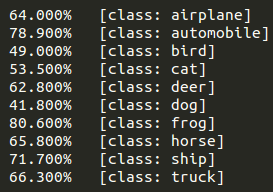
\includegraphics[width=1\textwidth]{\path/cifar-tanh.png} 
  \caption{Acc.= \textasciitilde 65\% f. di attivazione = TanH}
 \label{fig:training}
\end{subfigure}%
\begin{subfigure}{.5\textwidth}
  \centering
 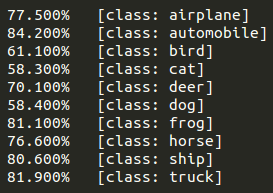
\includegraphics[width=1\textwidth]{\path/cifar-relu.png} 
  \caption{Acc.= \textasciitilde 73\% f. di attivazione = ReLU}
 \label{fig:validation}
\end{subfigure}
\caption{Percentuali di accuracy a seconda della funzione d'attivazione. La ReLU produce indubbiamente risultati migliori.}
\label{fig:relu}
\end{figure}
\end{comment}


\\
%%%%% NEW PAGE FOR THE NEW FIGURES %%%% 
\newpage
\pagebreak
\medskip
\newpage




 






%%%% forward pass con CPD %%% 
\begin{comment}
\begin{center}
\begin{align*}
	V(x, y, t) = \sum_i \sum_j \sum_s K(x-i, y-j, s, t)X(i, j, s) \\
		= \sum_r \sum_i \sum_j \sum_s K^x_r(x-i)K^y_r(y-i)K^s_r(s)K^t_r(t)X(i, j, s)\\
			= \sum_r K^t_r(t) \sum_i \sum_j K^x_r(x-i)K^y_r(y-i) \sum_s K^s_r(s) X(i, j, s) \tag{4}
\end{align*}
\end{center}
\end{comment}


